\chapter{Známe metódy detekcie prebalených aplikácií}
\label{chap:zname-metody}
Šírenie prebalených aplikácií predstavuje významnú hrozbu pre celý systém Android. Z~hľadiska bezpečnosti systému je v~súčasnosti detekcia prebalených aplikácií jednou z~najdôležitejších tém.
Téme prebalených APK súborov sa vo svojich prácach venuje viacero výskumných tímov. Bolo navrhnutých a implementovaných viacero spôsobov detekcie takýchto aplikácií. 
\newline 

\noindent Detekcia prebalených APK balíčkov vychádza z~nasledujúcich pozorovaní:
\begin{itemize}
	\item Prebalená aplikácia zachováva funkcionalitu pôvodnej aplikácie,
	\item Prebalená aplikácia zachováva vzhľad pôvodnej aplikácie,
	\item Prebalená a pôvodná aplikácia sú podpísané rôznymi entitami.
\end{itemize} 

\noindent Algoritmy detekcie prebalených aplikácií pozostávajú zvyčajne z~dvoch základných krokov:
\begin{itemize}
	\item Extrakcia vlastností aplikácií,
	\item Párové porovnanie aplikácií na základe extrahovaných vlastností.
\end{itemize}
\ \newline

\noindent Základným rozdielom medzi existujúcimi metódami detekcie prebalených APK súborov sú vlastnosti aplikácií použité pri detekcii malvérových duplikátov. Väčšia časť existujúcich algoritmov využíva podobnosť zdrojových kódov a inštrukcií. Existuje niekoľko metód, ktoré na detekciu prebalených aplikácií využívajú podobnosť multimediálnych súborov obsiahnutých v~APK balíčkoch.

\section{DroidMOSS}
Metóda \zv{DroidMOSS} je založená na podobnosti zdrojového kódu originálu a prebalenej kópie. Táto metóda sa zameriava na podobnosť aplikačného Java bytekódu a nezaoberá sa natívnym kódom. Počas prebaľovania je jednoduchšie modifikovať Java kód ako natívny kód a len malá časť aplikácií (približne 5 \%) používa natívny kód.

\zv{DroidMOSS} pozostáva z~troch kľúčových krokov. Prvým krokom je extrakcia aplikačných inštrukcií a získanie informácií o~vydavateľovi aplikácie v~podobe certifikátu. Tieto dva atribúty charakterizujú a odlišujú aplikácie.
Za účelom extrakcie aplikačného kódu je použitý nástroj \zv{smali/baksmali}, pomocou ktorého je súbor \zv{classes.dex} dekompilovaný do Dalvik bytekódu~\cite{smali}.  Počas procesu prebaľovania môže byť použitá obfuskácia kódu. Počas obfuskácie sú premenované názvy balíkov, tried, metód a premenných. \zv{DroidMOSS} sa s~obfuskáciou kódu vysporiadava pomocou ignorovania operandov. Pri tvorbe identifikátora aplikácie sú zohľadnené len operačné inštrukcie. Intuitívne môžeme tento prístup vysvetliť tak, že počas prebaľovania je jednoduché upraviť kód premenovaním premenných, oveľa náročnejšie je zmeniť kód tak, aby používal odlišné inštrukcie. 
Informácie o~autorovi aplikácie pochádzajú zo súborov v~adresári \cesta{META-INF}. \zv{DroidMOSS} vygeneruje identifikátor autora pomocou zahashovania verejného kľuča, mena vývojára a jeho kontaktných informácií. 

Druhý krok spočíva vo vygenerovaní unikátneho identifikátoru každej aplikácie. Hlavným dôvodom pre tvorbu identifikátoru je komplexnosť a veľký počet inštrukcií v~jednej aplikácii. Dĺžka identifikátoru je výrazne kratšia ako dáta o~inštrukciách aplikácie, čo umožňuje efektívnejšie porovnávanie aplikácií. 
Vytvorenie identifikátoru pomocou hashovania celého kódu aplikácie môže byť efektívne použité na overenie úplnej zhody dvoch aplikácií. Tento postup však nie je možné aplikovať pri určení podobnosti aplikácií.  Z~tohto dôvodu využíva \zv{DroidMOSS} špeciálnu hashovaciu techniku \zv{fuzzy hashing} \cite{fuzzyHashing}. Namiesto vytvorenia identifikátoru celej sekvencie inštrukcií je táto sekvencia najskôr rozdelená na kratšie časti. Následne je každá z~týchto častí hashovaná osobitne. Na vyhodnotenie podobnosti aplikácií sú použité identifikátory (hashe) týchto kratších sekvencií.

Posledným krokom je párové porovnanie aplikácií. Aplikácie sú  rozdelené do dvoch skupín. Jedna skupina obsahuje aplikácie z~\zv{Google Play Store}, druhá aplikácie z~neoficiálnych zdrojov.  \zv{DroidMOSS} využíva silný predpoklad, že aplikácie pochádzajúce z~\zv{Google Play Store} nie sú prebalené. 
Aplikácie z~rozdielnych skupín sú vzájomne porovnané. Na vyhodnotenie podobnosti je použitý algoritmus navrhnutý pomocou techniky dynamického programovania. Podobnosť aplikácií je určená ako minimálna vzdialenosť medzi identifikátormi dvoch sekvencií inštrukcií.  Vzdialenosť je reprezentovaná počtom úprav potrebných na pretvorenie identifikátora jednej sekvencie na identifikátor druhej sekvencie. Ak vypočítaná podobnosť presiahne definovanú hranicu a porovnávané aplikácie sú podpísané rôznymi vydavateľmi, aplikácia ktorá nepochádza z~\zv{Google Play Store} je označená za prebalenú. Použitá technika umožňuje efektívne lokalizovať zmeny vykonané v~prebalených aplikáciách. 

\begin{figure}[htb]
  \begin{center}
    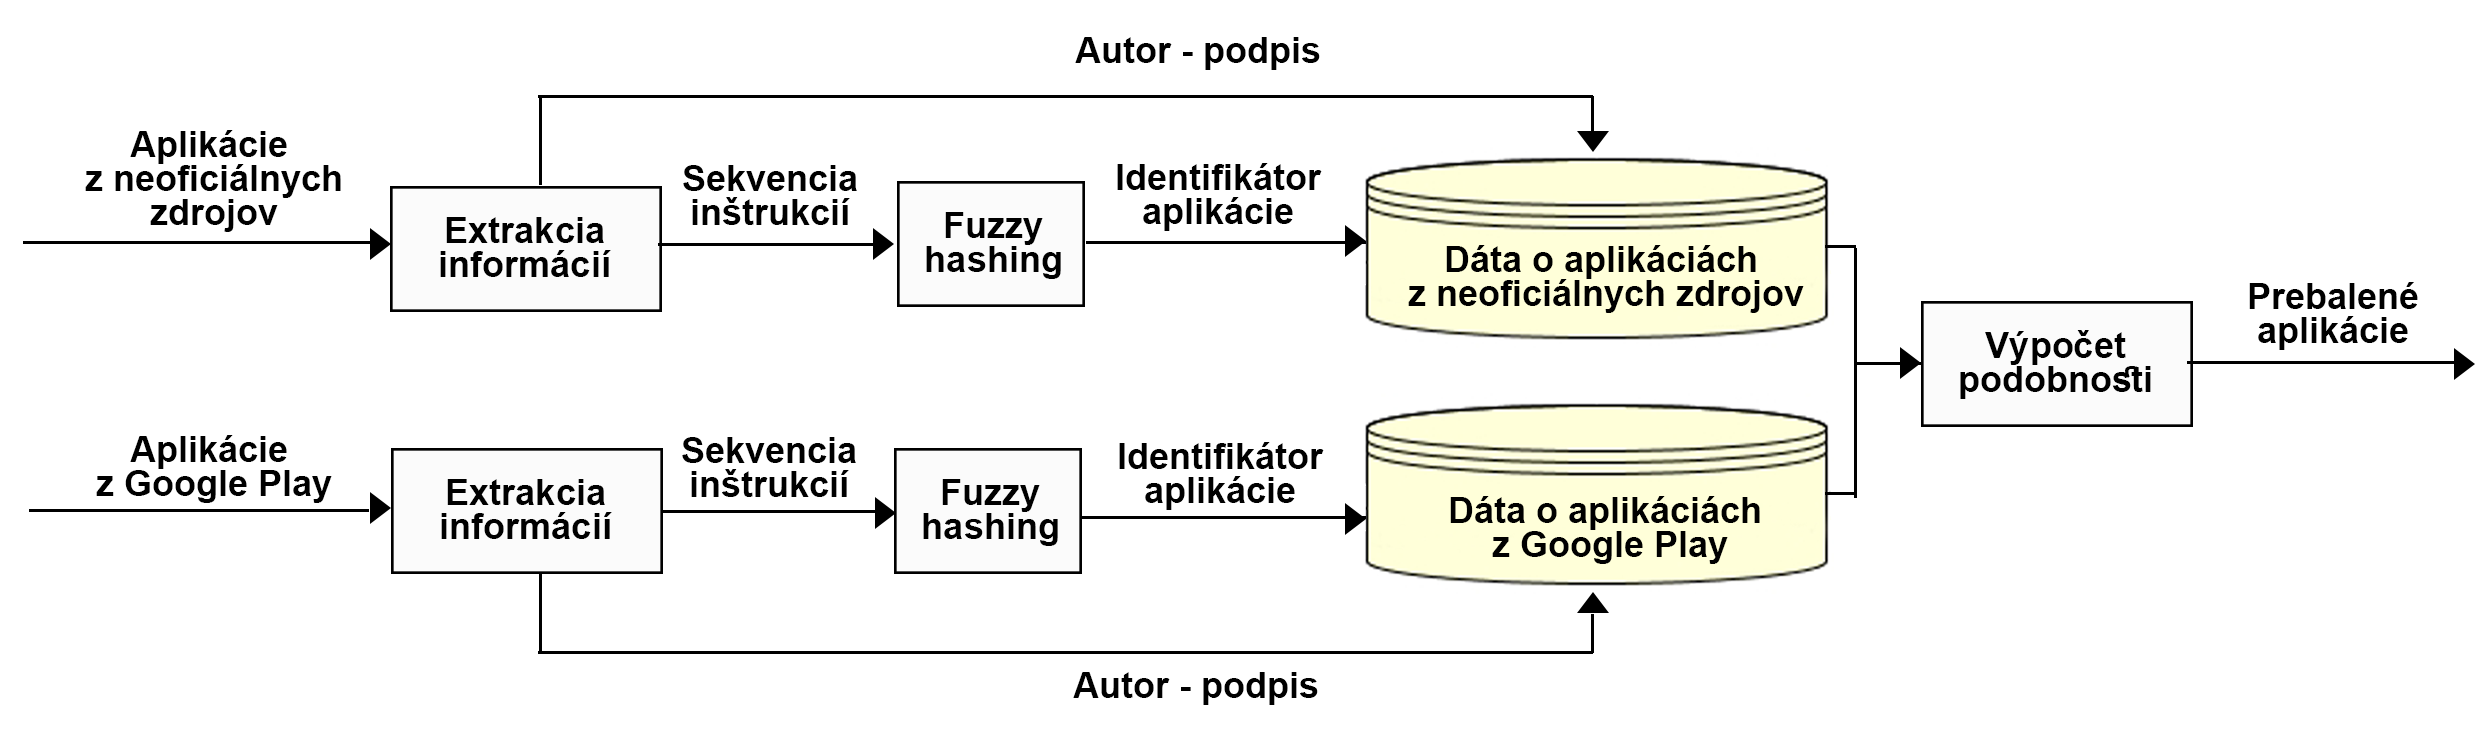
\includegraphics[width=130mm]{images/DroidMoss.png}
  \end{center}
  \caption{Postup metódy DroidMOSS}
  \label{fig:strukturaDroidMoss}
\end{figure}


Systém \zv{DroidMOSS} bol aplikovaný na kolekciu $86\,000$ aplikácií. Pomocou tejto techniky sa ukázalo, že $5$ až $13$ \% aplikácií distribuovaných pomocou alternatívnych zdrojov je prebalených~\cite{DetectingRepackagedZhou}.


\section{ImageStruct}

Metóda \zv{ImageStruct} používa pri detekcii prebalených aplikácií podobnosť obrázkových súborov. Tento spôsob je založený na pozorovaní, že podobné aplikácie (rôzne verzie tej istej aplikácie alebo prebalené aplikácie) obsahujú podobné obrázky, zatiaľ čo obrázky v~aplikáciách s~rôznou funkcionalitou sú rozdielne. 

\zv{ImageStruct} získava z~APK balíčka charakteristické dáta obrázkov. Na extrakciu obrázkových dát je použitý algoritmus \zv{pHash}. Tento algoritmus používa diskrétnu kosínusovú transformáciu, pomocou ktorej z~obrázka odstráni niektoré farebné frekvencie. To umožňuje detekciu podobnosti aj pri jednoduchších úpravách, ako napríklad zmena rozlíšenia alebo vystrihnutie časti obrazu~\cite{pHash}. Na identifikáciu vydavateľa sú použité údaje z~priečinka \cesta{META-INF}.


Extrahované dáta sú ukladané v~databáze \zv{Redis}, ktorá slúži ako rýchla cache pamäť. 
Podobnosť dvoch APK súborov je určená ako pomer spoločných obrázkov a všetkých obrázkov daných aplikácií.

\zv{ImageStruct}  porovnáva kolekciu aplikácií z~\zv{Google Play} s~aplikáciami z~alternatívnych obchodov, pričom využíva predpoklad, že \zv{Google Play} neobsahuje prebalené aplikácie. Ak hodnota podobnosti prekročí stanovenú hranicu a aplikácie sú podpísané rôznymi autormi, aplikácia z~alternatívneho zdroja je označená za prebalenú.
Nastavenie hodnoty hranice nad ktorou sú aplikácie považované za duplikáty je z~hľadiska presnosti a spoľahlivosti detekcie kľúčové. Autori uvádzajú, že pomocou viacerých experimentov určili túto hodnotu na $0,6$~\cite{ImageStruct}.

\begin{figure}[htb]
  \begin{center}
    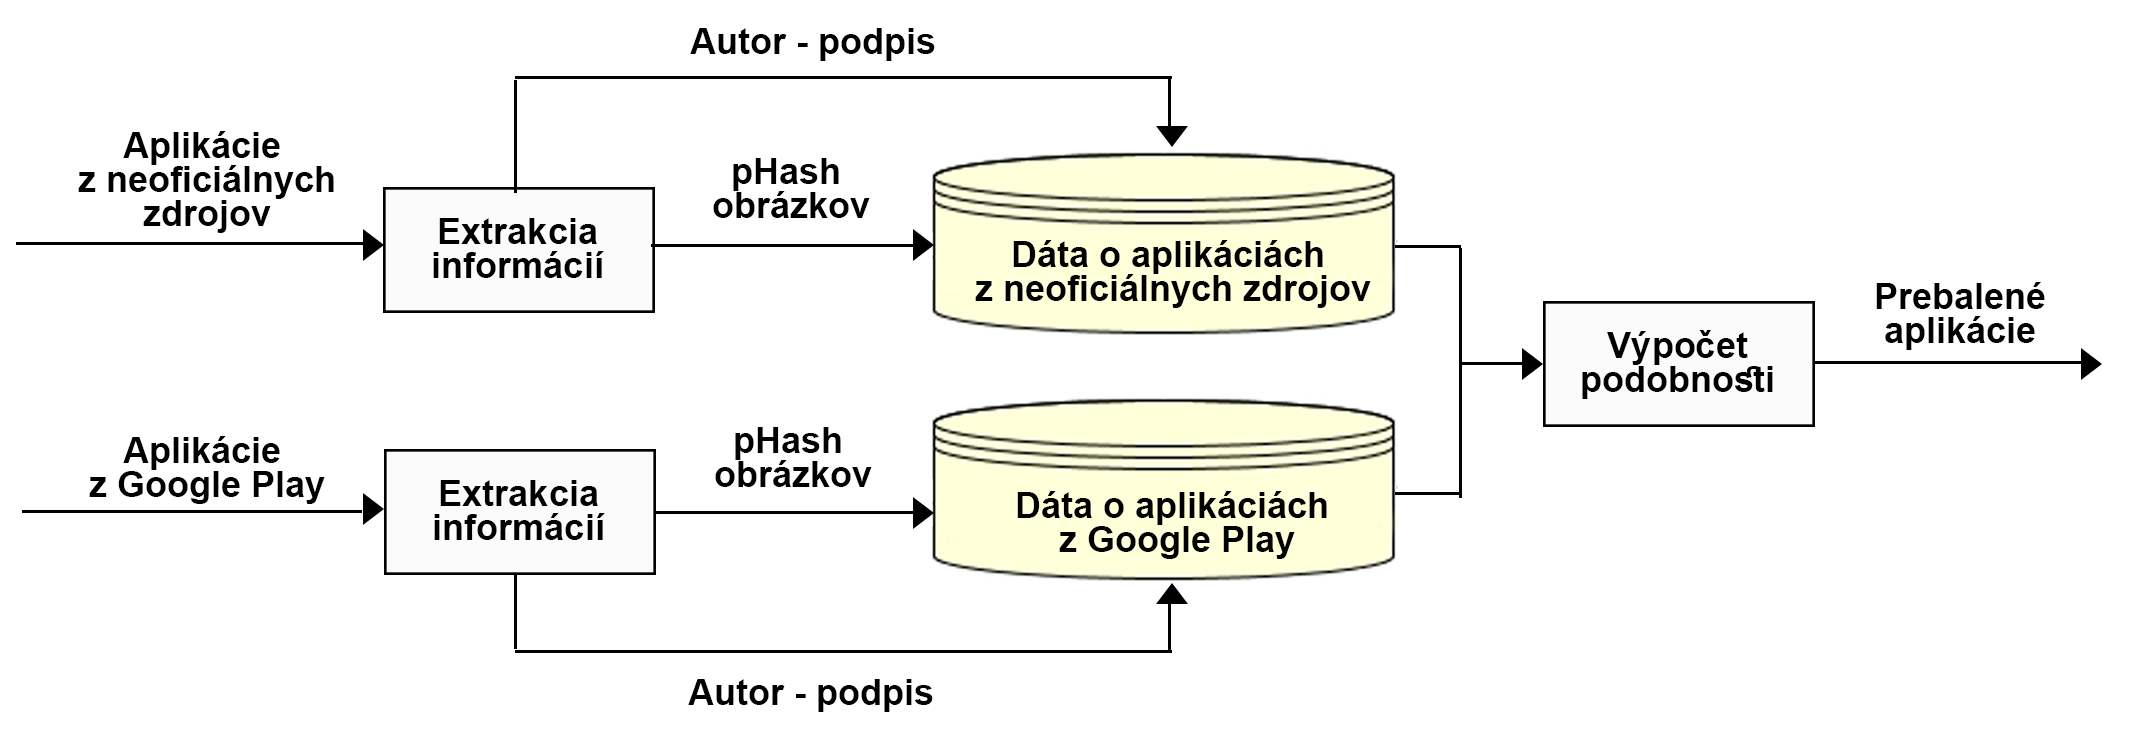
\includegraphics[width=130mm]{images/ImageStruct.png}
  \end{center}
  \caption{Postup metódy ImageStruct}
  \label{fig:strukturaImageStruct}
\end{figure}

Pomocou experimentov nad databázou $48\,000$ aplikácií z~\zv{Google Play} a alternatívnych zdrojov odhalila táto metóda, že výskyt prebalených aplikácií v~alternatívnych zdrojoch sa pohybuje medzi $6,7 \%$ až $14,5$ \%.
Pomer prebalených aplikácií detekovaných touto metódou je takmer rovnaký ako v~prípade metódy \zv{DroidMOSS}. Ako dôkaz použiteľnosti metód zameraných na podobnosť multimediálnych súborov bolo v~rámci experimentov vykonané porovnanie hodnôt podobnosti určených metódou \zv{ImageStruct} a metódou \zv{AndroGuard}, ktorá využíva podobnosť zdrojového kódu. Výsledky ukazujú, že medzi týmito postupmi existuje silná pozitívna korelácia~\cite{ImageStruct}. 


\section{FSquaDRA}
Základnou myšlienkou metódy \zv{FSquaDRA} je, že aplikácia obsahuje okrem zdrojového kódu a obrázkov aj množstvo iných súborov, ktoré definujú jej identitu. Preto táto metóda porovnáva všetky súbory dvoch aplikácií. Na evaluáciu podobnosti dvoch APK súborov je využitý Jaccardov index, ktorý sa určí ako pomer súborov, ktoré sa nachádzajú v~obidvoch balíčkoch, ku počtu súborov, ktoré sa nachádzajú v~aspoň jednej z~aplikácií.

Pri porovnaní súborov sú využité ich hashe vygenerované počas podpisu APK balíčka, ktoré sa nachádzajú v~súbore \cesta{MANIFEST.MF}. Využitie existujúcich hashov zefektívňuje túto metódu.
Rovnako ako pri ostatných metódach, aj \zv{FSquaDRA} využíva údaje z~adresára \cesta{META-INF} na identifikáciu vydavateľa aplikácie. 

Narozdiel od metód \zv{ImageStruct} a \zv{DroidMOSS} boli v~rámci experimentov porovnané všetky aplikácie medzi sebou. Hodnota Jaccardovho indexu, nad ktorou sú aplikácie považované za prebalené bola empiricky určená ako $0,7$.
Výsledky získané pomocou tejto metódy korešpondujú s~výsledkami získanými pomocou analýzy zdrojového kódu. V~porovnaní s~metódami založenými na analýze zdrojového kódu je tento spôsob oveľa rýchlejší. Autori uvádzajú, že za jednu minútu systém vykoná $1000$ párových porovnaní, zatiaľ čo metóda porovnávania zdrojového kódu vyhodnotí za rovnaký čas podobnosť jedného páru aplikácií.
Nevýhodou tejto metódy je, že neskúma obsah súborov a spolieha sa výhradne na ich hash. Pri prebaľovaní môže útočník mierne pozmeniť zdrojové súbory, čo má za následok znefunkčnenie detekcie~\cite{Zhauniarovich2014}. 

Použiteľnosť tejto metódy bola ďalej skúmaná v~práci \zv{Evaluation of Resource-Based App Repackaging
Detection in Android}~\cite{Gadyatskaya2016}. V~rámci tejto práce bola metóda vyhodnocovaná nad aplikáciami, ktoré obsahovali známe prebalené súbory, a teda bolo možné efektívne vyhodnotiť presnosť a úspešnosť tejto metódy. Práca potvrdila, že táto metóda je aj napriek nedostatkom dosahuje presnosť metód založených na analýze zdrojového kódu.